%\title{Presentation Template}
\documentclass[10pt]{beamer}

\usetheme[progressbar=frametitle]{metropolis}
\usepackage{appendixnumberbeamer}

\usepackage[compatibility=false]{caption}
\usepackage{subcaption}
\usepackage{csquotes}
\usepackage{booktabs}
\usepackage{hyperref}
\usepackage[scale=2]{ccicons}
\usepackage{tikz}
\usepackage{bm}

\usepackage{caption}
\captionsetup{justification=raggedright,singlelinecheck=false}

\usepackage{sidecap}
\sidecaptionvpos{figure}{c}

\usepackage{fontawesome}

\usepackage{footnpag} %reset footnotes at every page

\makeatother
\renewcommand{\thefootnote}{\ifcase\value{footnote}\or*\or
**\or***\or****\fi}
\makeatletter

\usepackage{xmpmulti}
\usepackage{pgffor}
\usepackage{multimedia}
\usepackage{media9}

\graphicspath{{./img/}}

\usepackage{pgfplots}
\usepgfplotslibrary{dateplot}

\usepackage{xspace}
\newcommand{\themename}{\textbf{\textsc{metropolis}}\xspace}

\definecolor{extralightgray}{gray}{0.85}

\title{Understanding Fraternal Transitions in Individuality}
\subtitle{OEE3 @ ALife 2018}
\date{July 25, 2018}
\author{Matthew Andres Moreno \newline \texttt{mmore500@msu.edu}}
\titlegraphic{\hfill\includegraphics[height=2cm]{img/MSU-Wordmark-Black}}

\usepackage{fix-cm}

\makeatletter\newcommand\HUGE{\@setfontsize\Huge{28}{34}}\makeatother

\begin{document}

\maketitle

% \begin{frame}{Table of contents}
%   \setbeamertemplate{section in toc}[sections numbered]
%   \tableofcontents[hideallsubsections]
% \end{frame}

\section{Background}

\begin{frame}{Why}

\begin{figure}
\includegraphics[width=0.5\textwidth]{blue-brain}
\caption{TODO \cite{trader_2014}}
\end{figure}

\end{frame}


\section{Selection on Kin Cooperating Group Structure}

\begin{frame}
\begin{itemize}
\item expect transition to occur
\item scalable
\item no simulation of ``realistic'' physics, abstract instead
\end{itemize}
\end{frame}

\begin{frame}{Resource Collection}
\begin{itemize}
\item need to anticipate
\item need to activate
\item communication with neighbors
\end{itemize}
\end{frame}

\begin{frame}{Channels, Signals, \& Resource}
\begin{itemize}
\item register into explicit cooperating groups called channels
\end{itemize}
\end{frame}

\begin{frame}{Channels, Signals, \& Resource}
\multiinclude[format=png,start=0,graphics={width=\textwidth}]{multichannel/frame}
\end{frame}

\begin{frame}{Signals \& Resource}
  \vspace{4ex}
  \begin{figure}
\begin{columns}
\begin{column}{0.5\textwidth}
    \foreach \n in {1,...,12}{%
    \includegraphics<\n>[width=\textwidth]{small_res/frame-\n.png}%
    }%
\end{column}
\begin{column}{0.5\textwidth}
    \foreach \n in {1,...,12}{%
    \includegraphics<\n>[width=\textwidth]{small_sig/frame-\n.png}%
    }%
\end{column}
\end{columns}%
\begin{columns}
\begin{column}{0.5\textwidth}
\begin{subfigure}[b]{\textwidth}
  \caption{resource}
\end{subfigure}
\end{column}
\begin{column}{0.5\textwidth}
\begin{subfigure}[b]{\textwidth}
\caption{activation-quiescence signals}
\end{subfigure}
\end{column}
\end{columns}
\caption{Co-visualization of same-channel signaling and resource distribution.}
\end{figure}

\end{frame}

\begin{frame}{Channel Inheritance}
  \vspace{8ex}
  \begin{figure}
\begin{columns}
  \begin{column}{0.5\textwidth}
    \colorbox{extralightgray}{\includegraphics[width=\textwidth]{same_channel_offspring}}
  \end{column}%
  \begin{column}{0.5\textwidth}
    \colorbox{extralightgray}{\includegraphics[width=\textwidth]{new_channel_offspring}}
  \end{column}%
\end{columns}%
\begin{columns}
  \begin{column}{0.5\textwidth}
    \begin{subfigure}[b]{\textwidth}
    \caption{Offspring inherits channel ID from parent.}
    \end{subfigure}
  \end{column}%
  \begin{column}{0.5\textwidth}
    \begin{subfigure}[b]{\textwidth}
    \caption{Offspring assigned new, unique channel ID.}
    \end{subfigure}
  \end{column}%
\end{columns}%
\caption{The two possible channel inheritance outcomes.}
\end{figure}

\end{frame}

\begin{frame}{Excluded Channel Dynamics}
  \vspace{6.6ex}
  \begin{figure}
\begin{columns}
  \begin{column}{0.5\textwidth}
\colorbox{extralightgray}{\hspace{0.136\textwidth}\includegraphics[width=0.728\textwidth,trim= 0 -83 0 -83]{plastic_channel}\hspace{0.136\textwidth}}
  \end{column}%
  \begin{column}{0.5\textwidth}%
\colorbox{extralightgray}{\includegraphics[width=\textwidth]{channel_collision_offspring}}
  \end{column}
\end{columns}%
\begin{columns}
  \begin{column}{0.5\textwidth}
    \begin{subfigure}[b]{\textwidth}
    \caption{during-lifetime channel change}
    \end{subfigure}
  \end{column}
  \begin{column}{0.5\textwidth}
    \begin{subfigure}[b]{\textwidth}
    \caption{non-inherited channel match\footnotemark}
    \end{subfigure}
  \end{column}
\end{columns}
\caption{Illustration of excluded channel dynamics.}
\end{figure}
\footnotetext{infrequent, non-inducible}

\end{frame}


\section{Hierarchical Extension}

\begin{frame}{Clumps \& Clumps of Clumps}

\vspace{4ex}

\begin{figure}
\begin{columns}
\begin{column}{0.05\textwidth}
\begin{subfigure}[b]{\textwidth}
\caption{}
\label{fig:natural}
\end{subfigure}
\end{column}
\begin{column}{0.27\textwidth}
\includegraphics[width=\textwidth]{cheek_cell}
\end{column}
\begin{column}{0.07\textwidth}
\includegraphics[width=\textwidth]{arrow}
\end{column}
\begin{column}{0.27\textwidth}
\includegraphics[width=\textwidth]{ant}
\end{column}
\begin{column}{0.07\textwidth}
\includegraphics[width=\textwidth]{arrow}
\end{column}
\begin{column}{0.27\textwidth}
\includegraphics[angle=270, width=\textwidth]{ant_bridge}
\end{column}
\end{columns}
\vspace{1ex}
\begin{columns}
\begin{column}{0.05\textwidth}
\end{column}
\begin{column}{0.27\textwidth}
\centering
cell {\tiny\cite{clare_and_ben_2017}}
\end{column}
\begin{column}{0.07\textwidth}
\end{column}
\begin{column}{0.27\textwidth}
\centering
ant {\tiny\cite{quinzani_2008}}
\end{column}
\begin{column}{0.07\textwidth}
\end{column}
\begin{column}{0.27\textwidth}
\centering
ant colony {\tiny\cite{gallice_2011}}
\end{column}
\end{columns}
\begin{columns}
\begin{column}{0.05\textwidth}
\end{column}
\begin{column}{0.27\textwidth}
\centering
\end{column}
\begin{column}{0.07\textwidth}
\end{column}
\begin{column}{0.27\textwidth}
\centering
(clump)
\end{column}
\begin{column}{0.07\textwidth}
\end{column}
\begin{column}{0.27\textwidth}
\centering
(clump of clumps)
\end{column}
\end{columns}
\vspace{2ex}
\begin{columns}
\begin{column}{0.05\textwidth}
\begin{subfigure}[b]{\textwidth}
\caption{}
\label{fig:simulated}
\end{subfigure}
\end{column}
\begin{column}{0.27\textwidth}
\includegraphics[width=\textwidth]{cell}
\end{column}
\begin{column}{0.07\textwidth}
{\Large$\underset{\phantom{\checkmark}}{\overset{\checkmark}{\includegraphics[width=\textwidth]{arrow}}}$}
\end{column}
\begin{column}{0.27\textwidth}
\includegraphics[width=\textwidth]{clump}
\end{column}
\begin{column}{0.07\textwidth}
{\Large$\underset{\phantom{?}}{\overset{\only<1,2>{?}\only<3>{\phantom{?}}}{\includegraphics[width=\textwidth]{arrow}}}$}
\end{column}
\begin{column}{0.27\textwidth}
\centering
\only<1,2>{\Large ?} \only<3>{\Large \phantom{?}}
\includegraphics[width=\textwidth]<2>{clumps}
\includegraphics[width=\textwidth]<3>{clump_of_clumps}
\end{column}
\end{columns}
\vspace{1ex}
\begin{columns}
\begin{column}{0.05\textwidth}
\end{column}
\begin{column}{0.27\textwidth}
\centering
cell
\end{column}
\begin{column}{0.07\textwidth}
\end{column}
\begin{column}{0.27\textwidth}
\centering
clump
\end{column}
\begin{column}{0.07\textwidth}
\end{column}
\begin{column}{0.27\textwidth}
\centering
\only<3>{\phantom{(}}\only<1,2>{(}clump of clumps\only<1,2>{)}\only<3>{\phantom{)}}
\end{column}
\end{columns}
\vspace{2ex}
\caption{Analogy between (\subref{fig:natural}) natural and (\subref{fig:simulated}) simulated hierarchical fraternal transitions of individuality.}

\end{figure}


\end{frame}


\begin{frame}{Clumps \& Clumps of Clumps}
\begin{figure}
\begin{columns}
  \begin{column}{0.5\textwidth}
    \includegraphics<1>[width=\textwidth]{hsvmap/hsvmap-clump}%
    \includegraphics<2>[width=\textwidth]{hsvmap/hsvmap-clump}%
    \includegraphics<3>[width=\textwidth]{hsvmap/hsvmap-clumpofclumps}%
    \includegraphics<4>[width=\textwidth]{hsvmap/hsvmap-clumpsofclumps}%
  \end{column}
  \begin{column}{0.5\textwidth}
    \includegraphics<1>[width=\textwidth]{channelviz/channelviz-cell}%
    \includegraphics<2>[width=\textwidth]{channelviz/channelviz-clump}%
    \includegraphics<3>[width=\textwidth]{channelviz/channelviz-clumpofclumps}%
    \includegraphics<4>[width=\textwidth]{channelviz/channelviz-clumpsofclumps}%
  \end{column}
\end{columns}
\begin{columns}
  \begin{column}{0.5\textwidth}
    \begin{subfigure}[b]{\textwidth}
    \caption{channel ID HSV key}
    \end{subfigure}
  \end{column}
  \begin{column}{0.5\textwidth}
    \begin{subfigure}[b]{\textwidth}
    \caption{channel map visualization}
    \end{subfigure}
  \end{column}
\end{columns}
\caption{Visualization of hierarchically-nested signaling networks.}
\end{figure}
\end{frame}


\begin{frame}{Signals \& Resource}
  \begin{figure}
\begin{columns}
\begin{column}{0.02\textwidth}
\rotatebox{90}{Level 2}
\end{column}
\begin{column}{0.49\textwidth}
    \centering
    \foreach \n in {1,...,12}{%
    \includegraphics<\n>[width=\textwidth,trim={0 0 0 250},clip]{big_res/frame-\n.png}%
    }%
\end{column}
\begin{column}{0.49\textwidth}
  \centering
  \foreach \n in {1,...,12}{%
  \includegraphics<\n>[width=\textwidth,trim={0 0 0 250},clip]{big_sig/frame-\n.png}%
  }%
\end{column}
\end{columns}%
\vspace{2ex}
\begin{columns}
\begin{column}{0.02\textwidth}
  \rotatebox{90}{Level 1}
\end{column}
\begin{column}{0.49\textwidth}
    \centering
    \foreach \n in {1,...,12}{%
    \includegraphics<\n>[width=\textwidth,trim={0 0 0 250},clip]{small_res/frame-\n.png}%
    }%
\end{column}
\begin{column}{0.49\textwidth}
  \centering
  \foreach \n in {1,...,12}{%
  \includegraphics<\n>[width=\textwidth,trim={0 0 0 250},clip]{small_sig/frame-\n.png}%
  }%
\end{column}
\end{columns}%
\begin{columns}
\begin{column}{0.02\textwidth}
\end{column}
\begin{column}{0.49\textwidth}
\begin{subfigure}[b]{\textwidth}
  \caption{resource}
\end{subfigure}
\end{column}
\begin{column}{0.49\textwidth}
\begin{subfigure}[b]{\textwidth}
\caption{activation-quiescence signals}
\end{subfigure}
\end{column}
\end{columns}
\caption{Co-visualization of same-channel signaling and resource distribution.}
\end{figure}

\end{frame}


\begin{frame}{Clumps of Clumps}
    % \multiinclude[format=png,start=0
    % ,graphics={width=\textwidth}]{multichannel/frame}
\end{frame}

\begin{frame}{Signals \& Resource: Level 2 {\small(Clumps of Clumps)}}
foo
\end{frame}

\begin{frame}{Multichannel Inheritance Outcomes}
  \begin{figure}
  \begin{subfigure}[b]{0.85\textwidth}
    \begin{columns}
    \begin{column}{0.05\textwidth}
      \caption{}~\\\vspace{0ex}~\\
      \label{fig:same_multichannel_offspring}
    \end{column}
    \begin{column}{0.95\textwidth}
      \colorbox{extralightgray}{\includegraphics[width=\textwidth]{same_multichannel_offspring}}
  \end{column}
\end{columns}
  \end{subfigure}
  \begin{subfigure}[b]{0.85\textwidth}
      \begin{columns}
      \begin{column}{0.05\textwidth}
        \caption{}~\\\vspace{0ex}~\\
        \label{fig:new_lowchannel_offspring}
      \end{column}
      \begin{column}{0.95\textwidth}
        \colorbox{extralightgray}{\includegraphics[width=\textwidth]{new_lowchannel_offspring}}
\end{column}
\end{columns}
  \end{subfigure}
  \begin{subfigure}[b]{0.85\textwidth}
      \begin{columns}
      \begin{column}{0.05\textwidth}
      \caption{}~\\\vspace{0ex}~\\
      \label{fig:new_highchannel_offspring}
      \end{column}
      \begin{column}{0.95\textwidth}
        \colorbox{extralightgray}{\includegraphics[width=\textwidth]{new_highchannel_offspring}\vspace{-10ex}}
\end{column}
\end{columns}
  \end{subfigure}
  \caption{
  Allowed multichannel inheritance outcomes;
  (\subref{fig:same_multichannel_offspring}) identical level 1 and 2 channels,
  (\subref{fig:new_lowchannel_offspring}) new level 1 channel with identical level 2 channel, and
  (\subref{fig:new_highchannel_offspring}) new level 1 and 2 channels.
  }
\end{figure}

\end{frame}

\begin{frame}{Signals \& Resource: Level 1 {\small(Clumps)} \& Level 2 {\small(Clumps of Clumps)}}%
  foo
\end{frame}


\appendix

\begin{frame}{For More Information}

\vspace{1ex}

{\HUGE\url{https://osf.io/n92c7/}}

\vspace{3ex}

\begin{itemize}
\item source code
\item data
\item figures and graphics
\item how-to-replicate tutorial
\item publication
\item slides
\item blog article
\end{itemize}

\end{frame}

\begin{frame}{People}

\vspace{1ex}

\begin{columns}
\begin{column}{0.25\textwidth}
  \centering
  \includegraphics[width=0.7\textwidth,trim={0 15 0 15},clip]{moreno}
\end{column}
\begin{column}{0.75\textwidth}
  \textbf{Matthew Andres Moreno}

  \href{https://twitter.com/MorenoMatthewA}{{\faTwitter} @MorenoMatthewA}

  \href{https://mmore500.github.io}{{\faGlobe} \texttt{https://mmore500.github.io}}

  \href{mailto: mmore500@msu.edu}{{\faEnvelope} \texttt{mmore500@msu.edu}}

\end{column}
\end{columns}

\vspace{1ex}

\begin{columns}
\begin{column}{0.25\textwidth}
  \centering
  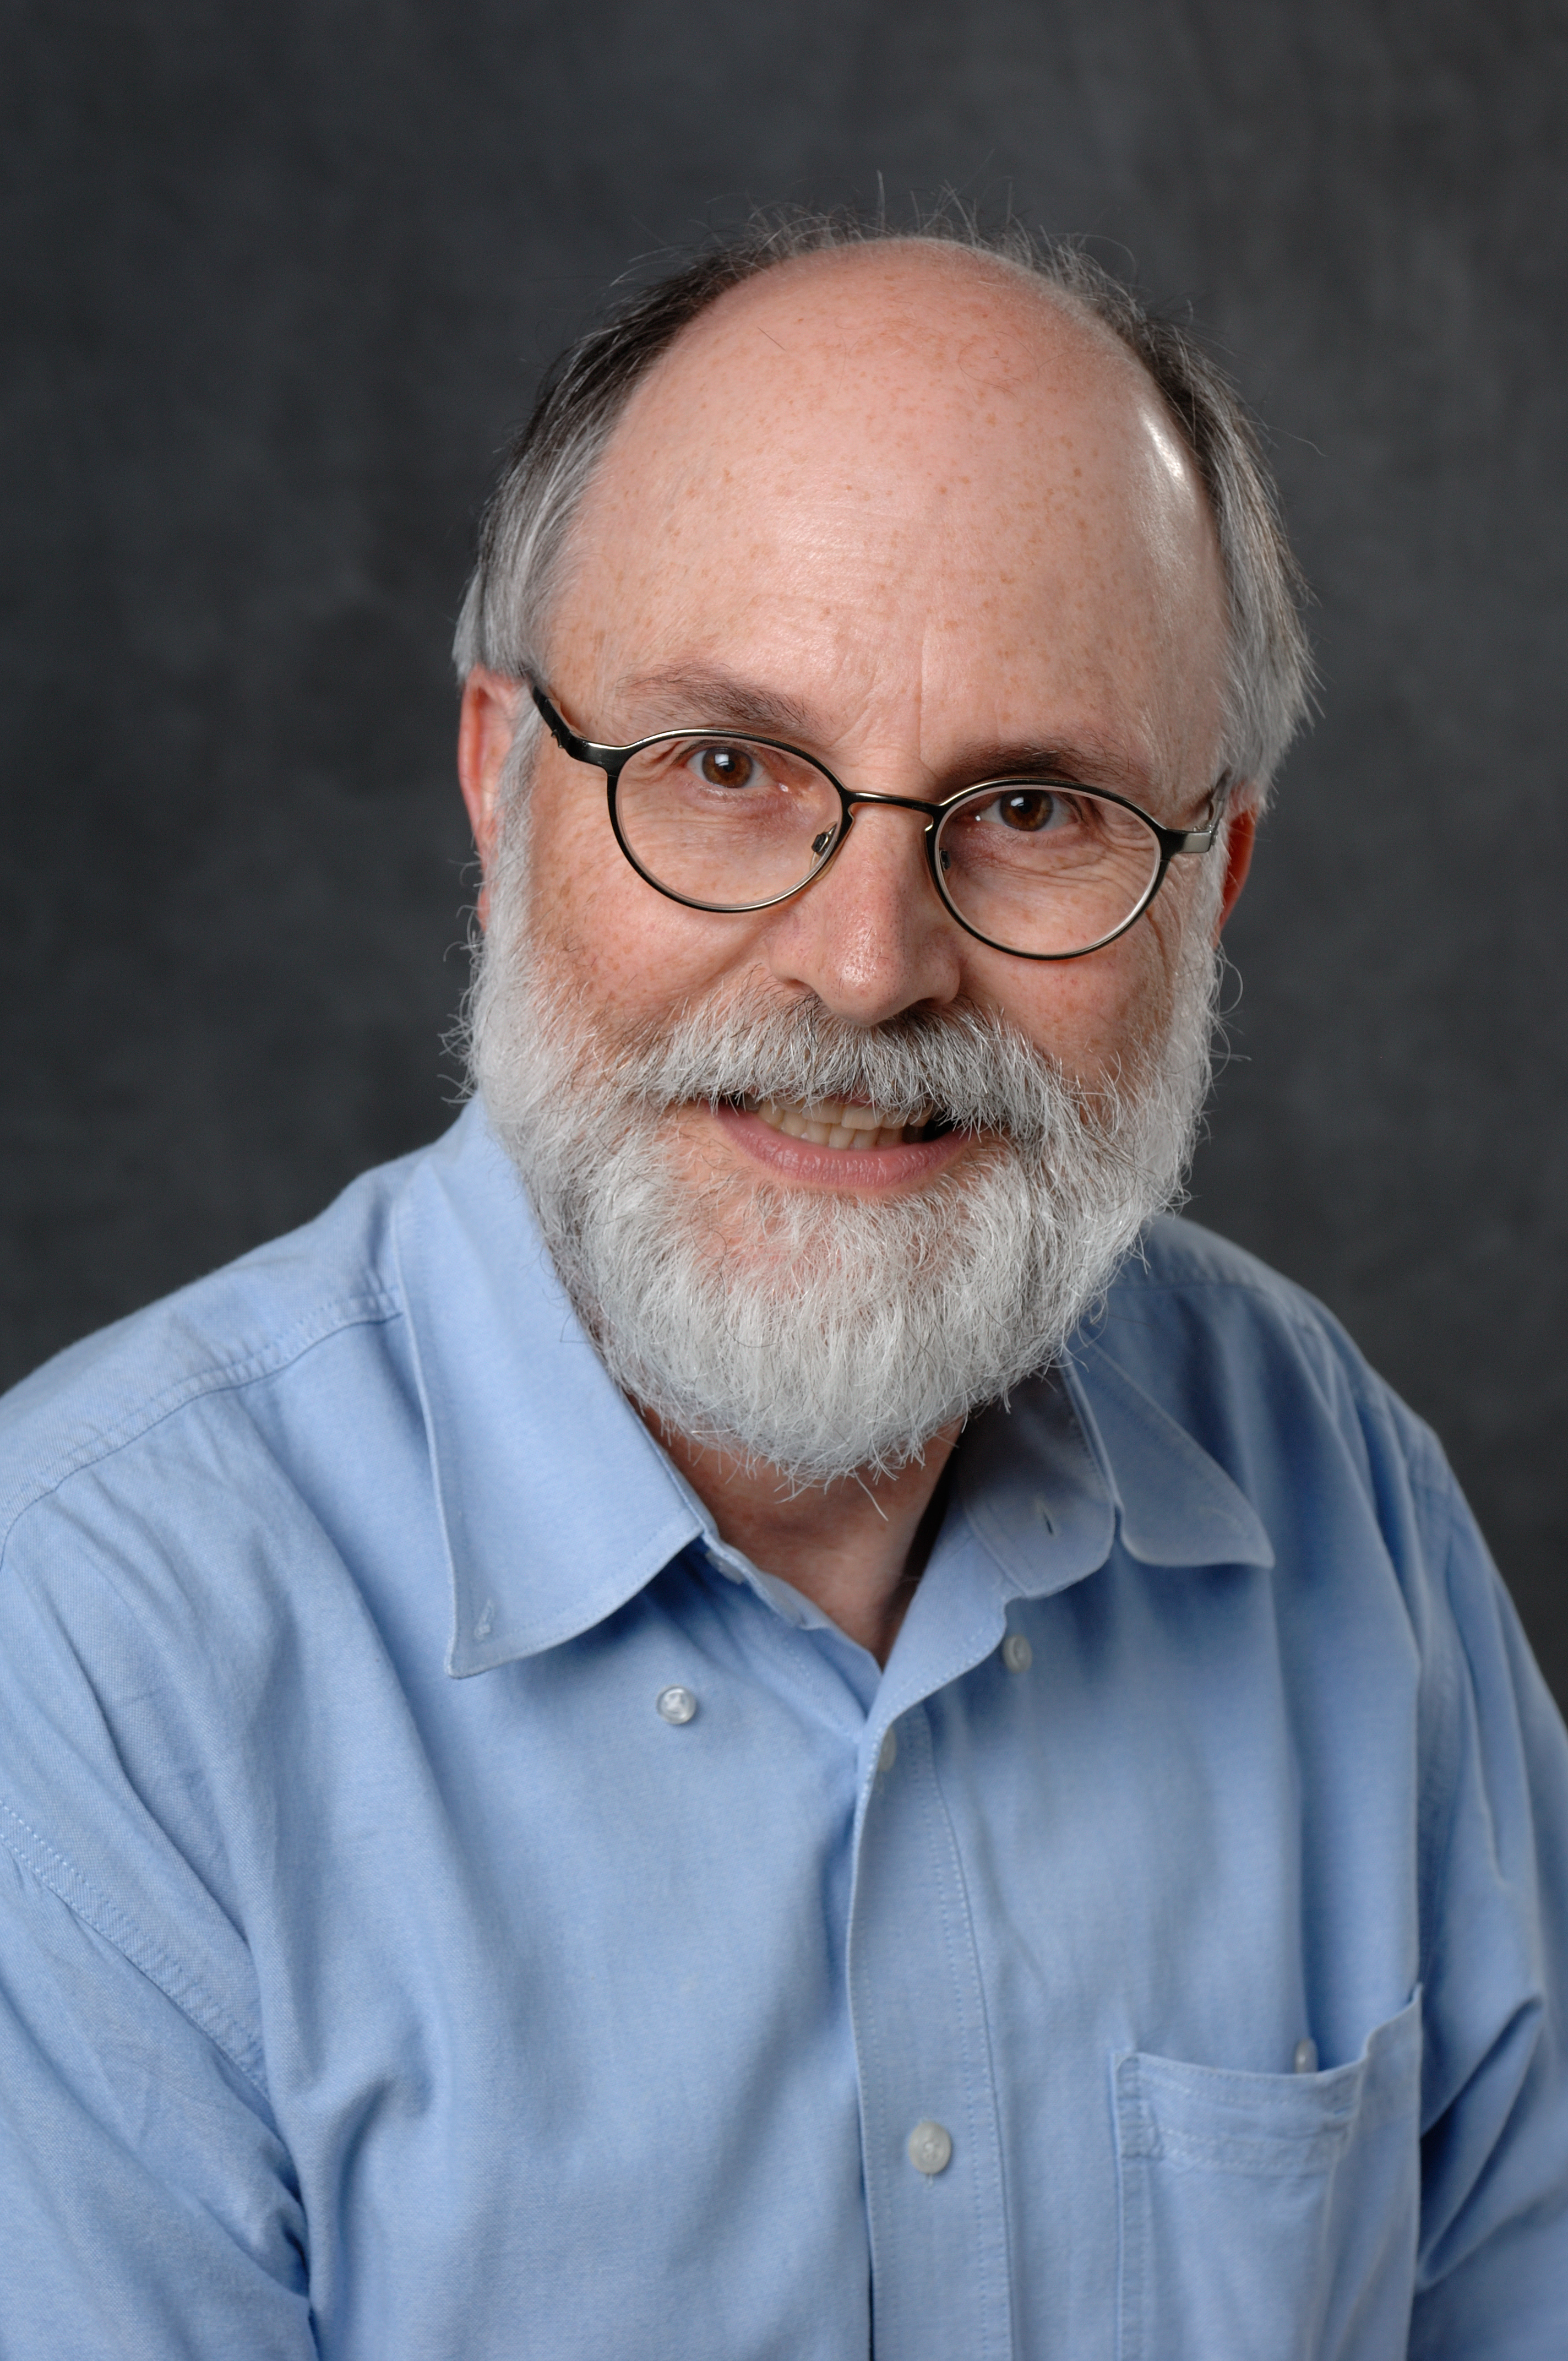
\includegraphics[width=0.7\textwidth,trim={0 100 0 50},clip]{banzhaf}
\end{column}

\begin{column}{0.75\textwidth}
  \textbf{Wolfgang Banzhaf}

  \href{http://www.cse.msu.edu/~banzhafw/}{{\faGlobe} \texttt{http://www.cse.msu.edu/\textasciitilde{}banzhafw/}}

  \href{mailto: banzhafw@msu.edu}{{\faEnvelope} \texttt{banzhafw@msu.edu}}

\end{column}
\end{columns}

\vspace{1ex}

\begin{columns}
\begin{column}{0.25\textwidth}
  \centering
  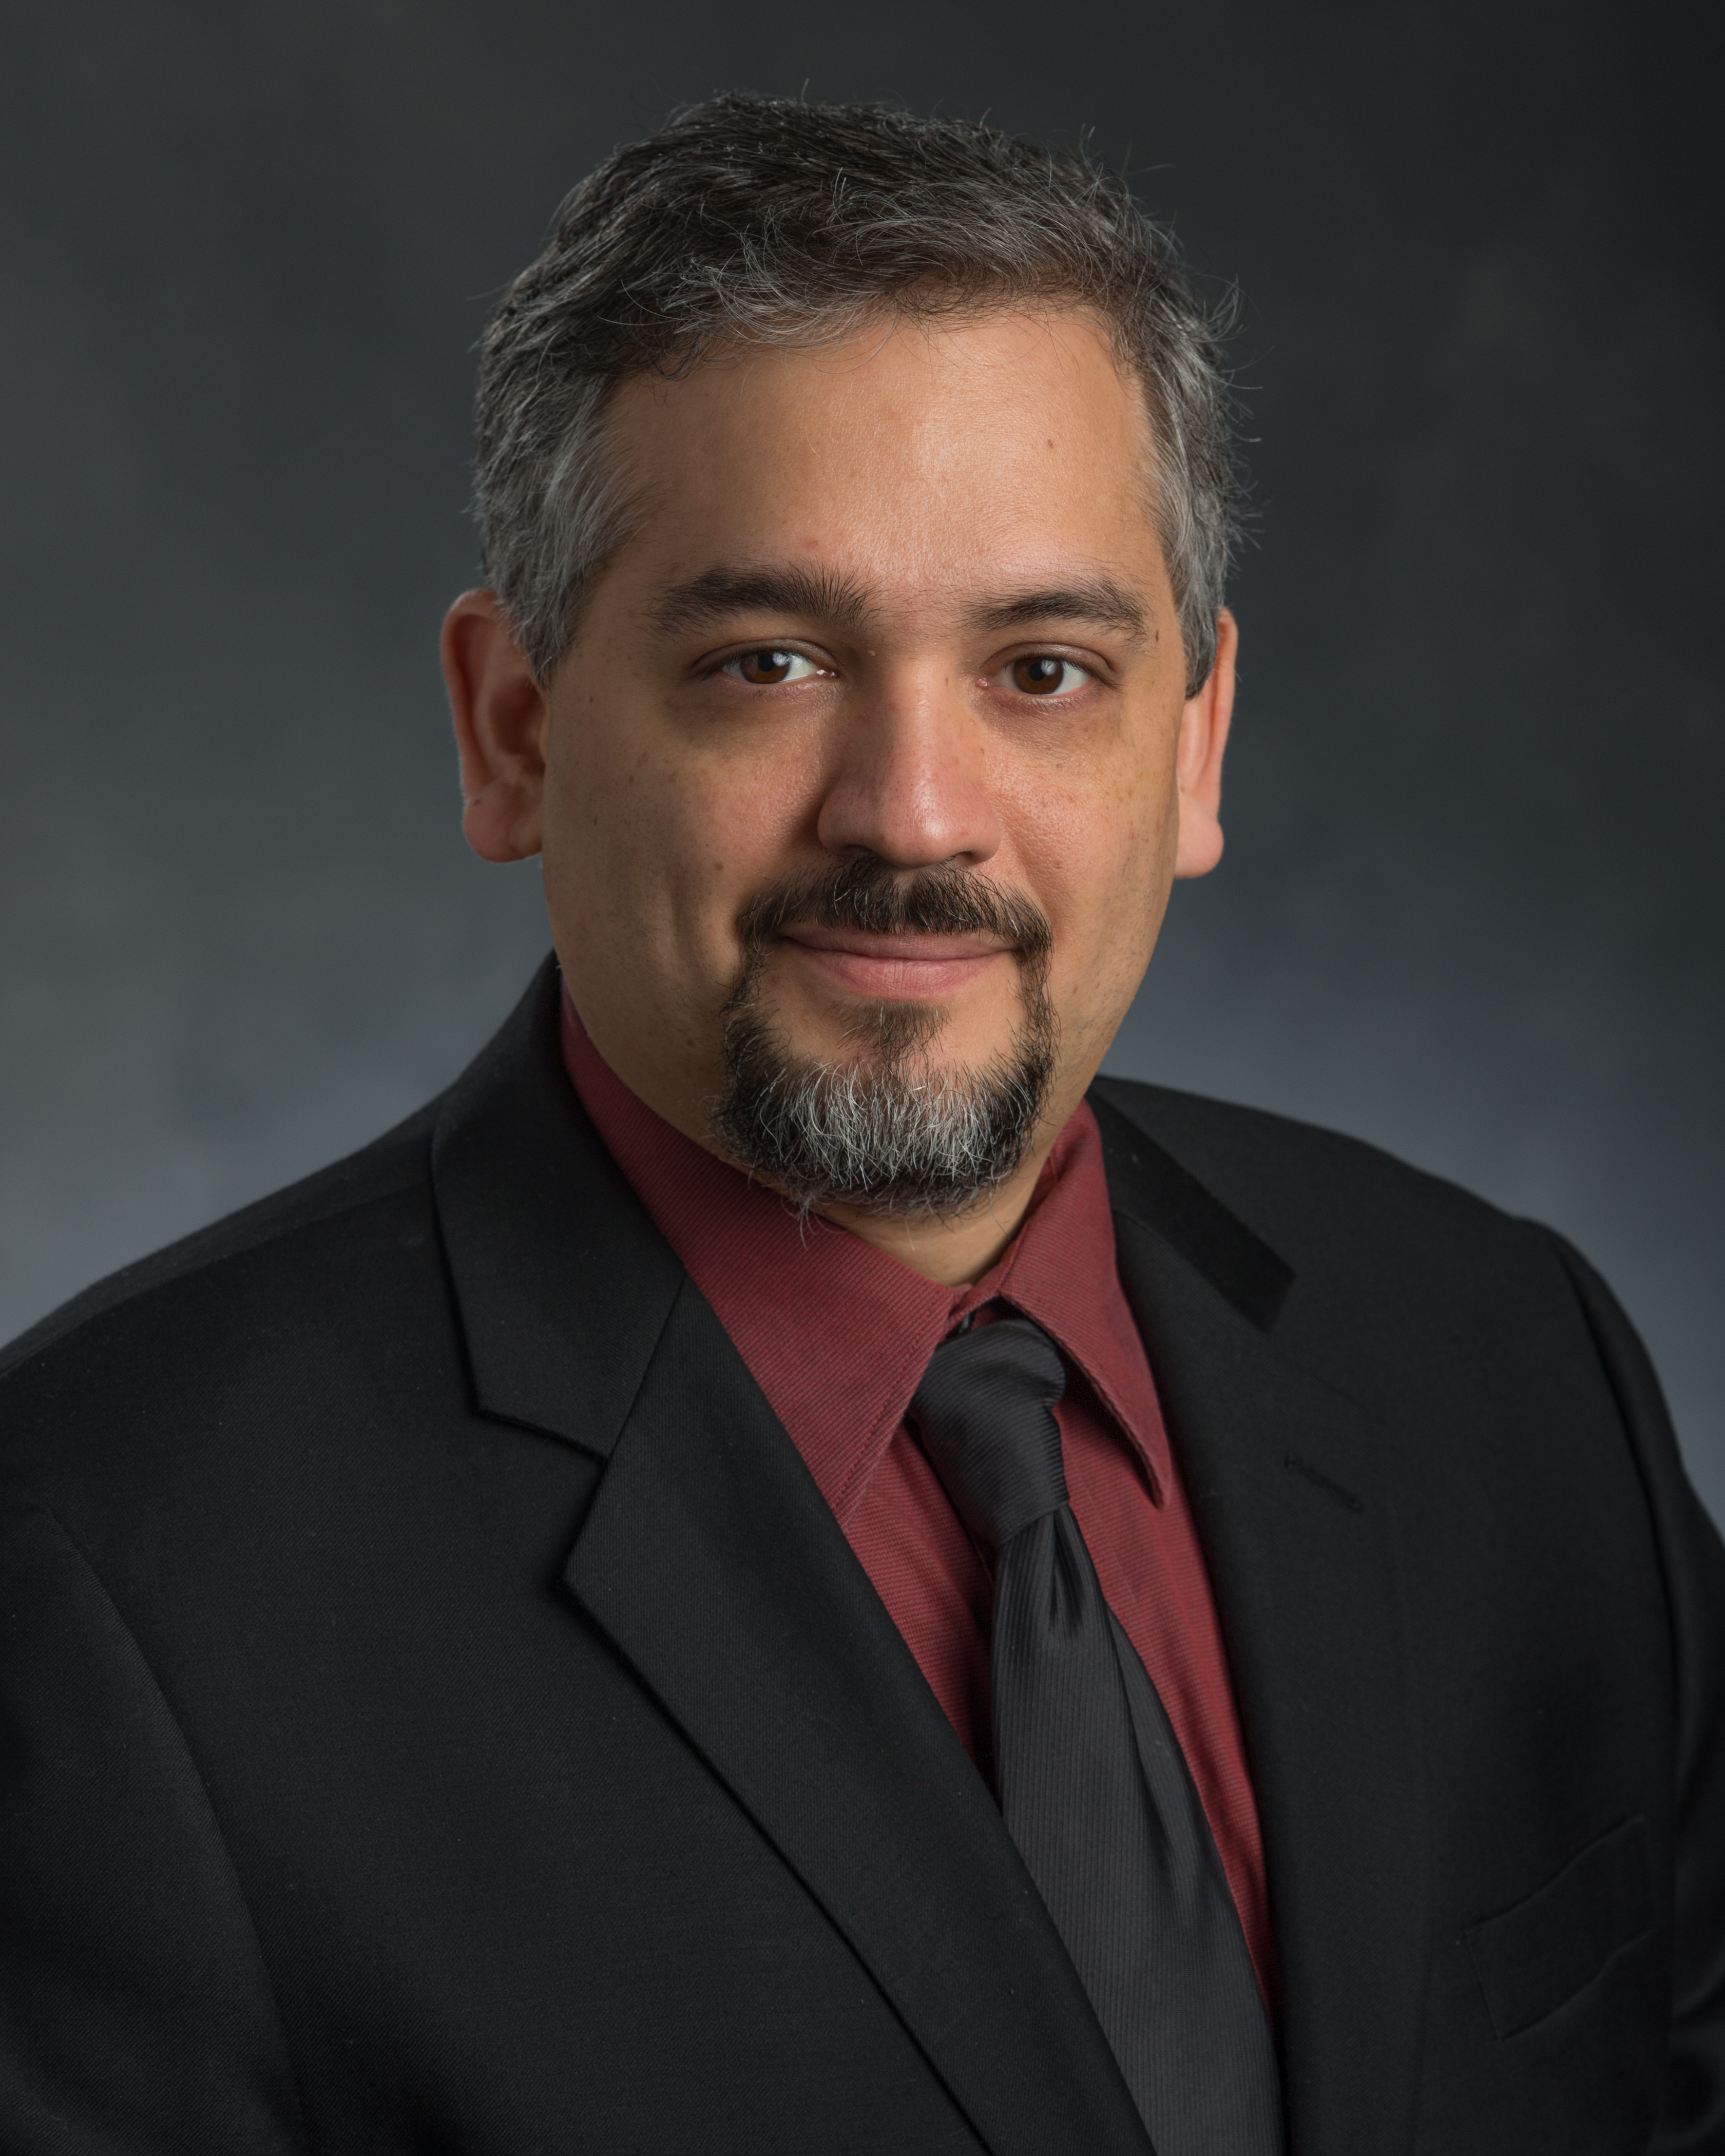
\includegraphics[width=0.7\textwidth]{ofria}
\end{column}

\begin{column}{0.75\textwidth}
  \textbf{Charles Ofria}

  \href{https://twitter.com/CharlesOfria}{{\faTwitter} @CharlesOfria}

  \href{https://ofria.com}{{\faGlobe} \texttt{https://ofria.com}}

  \href{mailto: ofria@msu.edu}{{\faEnvelope} \texttt{ofria@msu.edu}}

\end{column}
\end{columns}

\end{frame}

\begin{frame}{Acknowledgements}
\begin{itemize}
\item Distributed Evolutionary Algorithms for Python
package \cite{fortin2012deap}
\item PyTorch Deep Learning framework \cite{paszke2017pytorch}
\item Open Science Framework via the Center for Open Science
\item computational resources via Michigan State University's Institute for Cyber-Enabled Research
\item computational resources via Google Cloud Compute
\end{itemize}

\vfill

\newcommand{\innerspacer}{0.07\textwidth}
\newcommand{\content}{0.24\textwidth}
\newcommand{\outerspacer}{0.07\textwidth}

\begin{center}
 \begin{columns}
	\begin{column}{\outerspacer}~\end{column}
	 \begin{column}{\content}
		\includegraphics[width=\textwidth]{NSF-logo}
 	\end{column}
  \begin{column}{\innerspacer}~\end{column}
	 \begin{column}{\content}
		\includegraphics[width=\textwidth]{BEACON-logo}
 	\end{column}
  \begin{column}{\innerspacer}~\end{column}
 	\begin{column}{\content}
   \includegraphics[width=0.75\textwidth]{MSU-helmet}
 	\end{column}
 	\begin{column}{\outerspacer}~\end{column}
 \end{columns}
\end{center}

\end{frame}


\begin{frame}[standout]
  Questions?
\end{frame}

\begin{frame}[allowframebreaks]{References}

  \bibliography{bibl}
  \setbeamertemplate{bibliography item}{\insertbiblabel}
  \nocite{*} % Insert publications even if they are not cited in the poster
  \bibliographystyle{apalike}
\end{frame}


% \begin{frame}{Scrabble Result: Evolvability Signature}

\begin{figure}
  \includegraphics[width=0.8\linewidth]{img/results/scrabble_es_kde}
  \caption{
    Gaussian kernel density estimates for evolvability signatures of direct and indirect encodings in Scrabble string domain.
  }\label{fig:scrabble_es_kde}
\end{figure}


\end{frame}

\begin{frame}{Toy Result: Evolvability Signature}

\begin{figure}
  \begin{subfigure}[b]{0.33\linewidth}
    \includegraphics[width=\linewidth]{img/results/direct_es_unscaled}
    \subcaption{
      direct map
    }\label{fig:table_direct_es}
  \end{subfigure}
  \begin{subfigure}[b]{0.33\linewidth}
    \includegraphics[width=\linewidth]{img/results/noise_es_unscaled}
    \subcaption{
      denoising map
    }\label{fig:table_noise_es}
  \end{subfigure}
  \begin{subfigure}[b]{0.33\linewidth}
    \includegraphics[width=\linewidth]{img/results/bottleneck_es_unscaled}
    \subcaption{
      bottleneck map
    }\label{fig:table_bottleneck_es}
  \end{subfigure}
  \caption{
    Evolvability signatures for three genotype-phenotype maps in the $n$-legged table problem domain.
    Note that subfigure \ref{fig:table_bottleneck_es} is presented with different axis scaling than subfigures \ref{fig:table_direct_es} and \ref{fig:table_noise_es}.
  }\label{fig:all_es}
\end{figure}


\end{frame}

\begin{frame}{Evolutionary Algorithm Parameters: Toy Problem}

\begin{itemize}
\item population size: 300
\item tournament selection: $k = 5$
\item crossover: two-point, two-parent, $p = 0.5$
\item mutation: site-wise Gaussian perturbation
\begin{itemize}
\item training data, evolvability-signature experiments: $\mu = 0$, $\sigma = 0.1$, per-individual
probability = 0.2, per-site probability = 0.01
\item response-to-selection experiments: $\mu = 0$, $\sigma = 0.1$, per-individual probability = 0.2, per-site probability = 0.2 %TODO check this
\footnote{for the bottleneck map, a per-site probability of 1 was employed}
\end{itemize}
\end{itemize}

\end{frame}

\begin{frame}{Denoising Autoencoder Hyperparameters: Toy Problem}

\begin{itemize}
\item 100-to-100 fully-connected linear layer without bias
\item trained for 2500 epochs by stochastic gradient descent
\item learning rate: $10^{−4}$
\item momentum: 0.9
\item batch size: 2048
\item model parameters initialized uniformly between 0.005 and 0.015
\item model parameters clamped in the range (0, 1
\item during the training process, Gaussian
  noise with $\mu = 0$, $\sigma = 0.025$ applied to input
\item loss: mean square error of the difference between the original phenotype the reconstructed phenotype
\end{itemize}

\end{frame}

\begin{frame}{Evolutionary Algorithm Parameters: Scrabble Problem}

TODO

\end{frame}


\end{document}
